\chapter{平面电磁波}
\label{chap:plane wave}

本章讨论无限或半无限介质中的平面波。首先论述了平面电磁波在非导电介质中的基本性质：平面电磁波的横向性、线偏振态和圆偏振态。然后推导了至关重要的电磁波在平面分界面上反射和折射的Fresnel公式，并加以应用，接着概括阐述了电介质、导体和等离子体的高频色散关系。%对200赫兹以上各种频率的电磁波画出了液态水的折射率和吸收系数对频率的关系曲线(图7.9),通过全面的图象分析，说明了许多性质。
而后简单地讨论了电磁波在电离层中的传播，和在导电介质或耗散介质中的波。继而介绍了相速度和群速度的概念，以及一个脉冲或波包在色散介质中传播时的扩展。%相当详细地讨论了因果性这一重要课题，以及由此而得到的有关介质色散性质的一些结果，包括 Kramers--Kronig 色散关系以及根据这些关系导出的各种求和法则.本章最后论述了关于信号在色散介质中的传播这一经典问题，此问题最早是由 Sommerfeld 和 Brillouin（1914年）讨论过的，但只不过在最近才获得了实验的验证.

\section{非导电介质中的平面波}

电磁场Maxwell方程组的基本特征是存在行波解，这些解描写能量从一点输运到另一点.最简单最基本的电磁波是横平面波。%我们首先考虑在简单的(即$\varepsilon,\mu$是常数)非导电介质这种情形下如何求得这些解。

% 当没有源存在时，无限介质中的Maxwell方程组是：
% \begin{alignat*}{2}
%     \div\bm D&=0,&\qquad\curl\bm E+\pv{\bm B}t&=\bm 0,\\
%     \div\bm B&=0,&\curl\bm H-\pv{\bm D}t&=\bm 0.
% \end{alignat*}

考虑无源介质($\rho = 0,\;\bm J = \bm 0$)，并假设场是随时间简谐的($\e^{-\i\omega t}$)，Maxwell方程为
\begin{subequations}
    \begin{align}
        \div\bm D &= 0,\\
        \div\bm B &= 0,\\
        \curl\bm E &= \i\omega\bm B,\\
        \curl\bm H &= -\i\omega\bm D.
    \end{align}
\end{subequations}
对于均匀各向同性的线性介质，
\begin{align*}
    \bm D &= \varepsilon\bm E,\\
    \bm B &= \mu\bm H,
\end{align*}
%进一步假设没有色散，即$\varepsilon,\mu$是不随时间变化的正实数(无损耗)，可以得到
可以推出，$\bm E,\bm H$均满足如下的Helmholtz波动方程：
\begin{equation}
    (\laplacian + k^2)\begin{Bmatrix}
        \bm E\\\bm H
    \end{Bmatrix} = 0,
\end{equation}
其波数(wave number)定义为
\begin{equation}
    k = \sqrt{\mu\varepsilon}\omega.
\end{equation}

Helmholtz方程的一个解是沿$z$方向传播的平面波$\e^{\i(kz-\omega t)}$，其
相位为$\varphi = kz - \omega t$，等相位面移动的速度称为
相速度(phase velocity)：
\begin{equation}
    v_\varphi := \frac{\omega}k = \frac1{\sqrt{\mu\varepsilon}} = \frac{c}{\sqrt{\mu_\relative\varepsilon_\relative}}.
\end{equation}
% 对于非色散介质，$\varepsilon,\mu$与频率无关，有通解
% \[
%     u(x,t)=f(x-vt)+g(x+vt).
% \]

\paragraph{平面电磁波}

频率为$\omega$、波数为$k$、传播方向为$\uvec n$的平面电磁波一般具有如下形式：
\begin{equation}
    \begin{cases}
        \bm E = \bm E_0\e^{\i(\bm k\cdot\bm r-\omega t)},\\
        \bm B = \bm B_0\e^{\i(\bm k\cdot\bm r-\omega t)},
    \end{cases}
\end{equation}
其中$\bm E_0,\bm B_0$是常矢量，$\bm k := k\uvec n$为波矢(wave vector)。
\begin{theorem}{}{}
    无源Maxwell方程组与下列方程组等价
    \begin{subequations}
        \begin{align}
            \laplacian\bm E + k^2\bm E &= \bm 0,\\
            \div\bm E &= 0,\\
            \curl\bm E &= \i\omega\bm B.
        \end{align}
    \end{subequations}
\end{theorem}
\begin{corollary}
    电磁波是横波(transverse wave)，即$\bm E,\bm B$均垂直于传播方向$\uvec n$：
    \begin{subequations}
        \label{eqn:transverse}
        \begin{align}
            \bm k \cdot \bm E_0 &= 0,\\
            \bm k \cdot \bm B_0 &= 0,\\
            \bm k \times \bm E_0 &= \omega\bm B_0.
        \end{align}
    \end{subequations}
    同时$\uvec n \cdot \uvec n = 1$，注意：$\uvec n$可以是复矢量，此时$\abs{\uvec n}^2 = \uvec n \cdot \uvec n^* \neq 1$。
\end{corollary}

\paragraph{实波矢}

在普通透明介质（$\varepsilon,\mu > 0$）中，若$\uvec n$为实矢量，$\bm B_0 = (k/\omega)\uvec n \times \bm E_0$。以线偏振为例，电场和磁场同相，且可写成
\begin{subequations}
    \begin{align}
        \bm E_0 &= E_0\uvec\epsilon_1,\\
        \bm B_0 &= \sqrt{\mu\varepsilon}E_0\uvec\epsilon_2.
    \end{align}
\end{subequations}
其中
$\uvec n,\uvec\epsilon_1,\uvec\epsilon_2$是两两正交的单位矢量。
$\uvec n$称为传播矢量(propagation vector)，
$\uvec\epsilon_1,\uvec\epsilon_2$称为极化矢量(polarization vector)。

由复Poynting矢量的实部可得沿传播方向的周期平均能流，
\begin{equation}
    \ave{\bm S} = \frac12\Re(\bm E_0 \times \bm H_0\conj)
       = \frac12\sqrt{\frac{\varepsilon}{\mu}}\abs{\bm E_0}^2\uvec n .
\end{equation}
若本构参数在波包的频带内还可以视为与频率无关，则电、磁场分别贡献一半周期平均储能，
\begin{equation}
    \ave u = \frac14\biggp{\varepsilon\abs{\bm E_0}^2 + \frac1\mu\abs{\bm B_0}^2}
          = \frac{\varepsilon}{2}\abs{\bm E_0}^2 .
\end{equation}
在这些条件下，能量速度$\abs{\ave{\bm S}}/\ave u$等于相速度$v_\varphi$。透明色散介质则须计入材料的储能，见\eqref{eqn:Brillouin energy}和下文的\exmref{exm:plasma energy speed}。

\paragraph{复波矢}

若$\uvec n$是复矢量，
% 分成实部和虚部两部分：
% \[
%     \uvec n=\Re(\uvec n)+\i\Im(\uvec n),
% \]
则电磁波为非均匀平面波，在虚部方向$\Im(\uvec n)$上呈指数衰减(或增长)
\[
    \e^{\i(\bm k\cdot\bm r-\omega t)} = \e^{-k\Im(\uvec n)\cdot\bm r}\e^{\i(k\Re(\uvec n)\cdot\bm r-\omega t)},
\]
等幅面和等相面仍然是平面，但它们不再平行；横波的关系\eqref{eqn:transverse}仍成立，由$\uvec n \cdot \uvec n = 1$：
\begin{subequations}
    \begin{align}
        \abs{\Re(\uvec n)}^2 - \abs{\Im(\uvec n)}^2 &= 1,\\
        \Re(\uvec n) \cdot \Im(\uvec n) &= 0.
    \end{align}
\end{subequations}

\section{偏振}

前文指出：均匀平面波的电场沿$\uvec\epsilon_1$方向，磁场沿$\uvec\epsilon_2$方向；但显然，一旦确定极化矢量$\uvec\epsilon_1,\uvec\epsilon_2$后，一个均匀平面波的电场当然也可以沿其他方向，一般地，
可以将任意均匀平面波分解成两种偏振方向的波：
%也可以有一种平面波的电场$\uvec\epsilon_2$方向，
%我们分别称其为偏振矢量为$\uvec\epsilon_{1,2}$的线偏振波，这两种偏振波是不同的。一般地，
\[
    \bm E = (E_1\uvec\epsilon_1 + E_2\uvec\epsilon_2)\e^{\i(\bm k\cdot\bm r-\omega t)},
\]
振幅$E_1,E_2$是复数，$E_2$相对$E_1$的相位差为$\delta$。
% 因为$t$的起始点是任意的，不妨令$E_1$是实数，则$E_2=\abs{E_2}\e^{\i\delta}$。
% \[
%     E_1=a_1\e^{\i\delta_1},\quad E_2=a_2\e^{\i\delta_2}.
% \]
% 若选定$(\uvec n,\uvec\epsilon_1,\uvec\epsilon_2)=(\uvec z,\uvec x,\uvec y)$，取实部得到
% \begin{align*}
%     E_x&=a_1\cos(kz-\omega t+\delta_1),\\
%     E_y&=a_2\cos(kz-\omega t+\delta_2).
% \end{align*}

\paragraph{线偏振}

若$E_1,E_2$同相($\delta = 0,\ang{180}$)，则$\bm E$是线偏振的(linear polarized)。%$\bm E$与$\uvec\epsilon_1$的夹角是不变的，
%在$\uvec\epsilon_1,\uvec\epsilon_2$坐标系中，
如\figref{fig:linear polarization}，
$\bm E$的终点在一条直线(图中虚线)上简谐运动。
细箭头表示$\bm E$终点运动方向，
\begin{notecaptionblock}
	\tikzfigure{linear-polarization}
    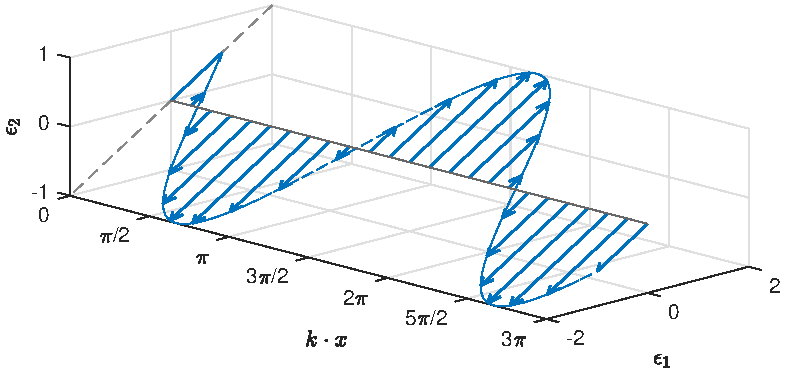
\includegraphics[width=0.5\linewidth]{figures/polarization_line.pdf}
	\captionof{figure}{线偏振($\delta = 0$)。本节三幅偏振波形图中的两个横向电场分量均以同一参考场强 $E_{\mathrm{ref}}$ 归一化。}
    \label{fig:linear polarization}
\end{notecaptionblock}

\paragraph{圆偏振}

若$E_1,E_2$不同相，但幅值相同($\abs{E_1} = \abs{E_2}$)且相位差$\delta = \pm\ang{90}$，则
$\bm E$是圆偏振的(circular polarized)，可以写成
\[
    \bm E = E_1(\uvec\epsilon_1 \pm \i\uvec\epsilon_2)\e^{\i(\bm k\cdot\bm r-\omega t)},
\]
如\figref{fig:circular polarization}，向$-\bm k$方向(即垂直纸面向内)看去，($+$)对应电场终点逆时针(counterclockwise)旋转，我们称为左旋(left circular)或正螺旋性(positive helicity)，因为其角动量是沿$+\bm k$的；相应的，($-$)对应顺时针旋转，称为右旋或负螺旋性。
\begin{notecaptionblock}
    \tikzfigure{circular-polarization}
    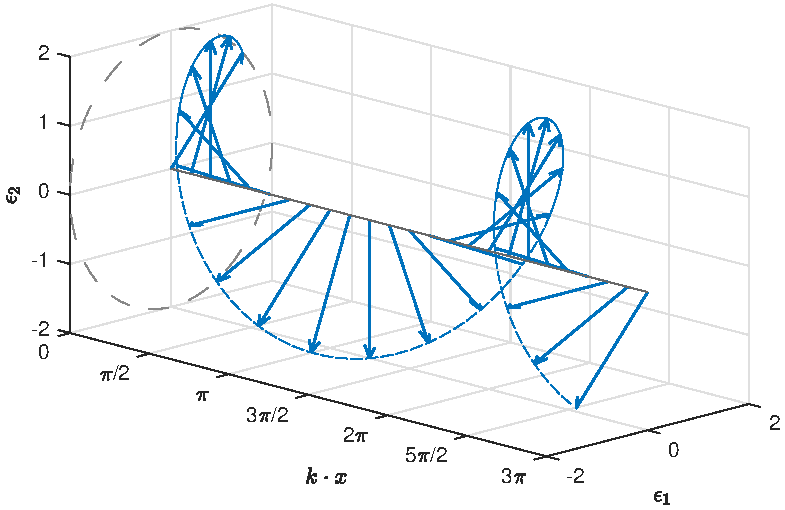
\includegraphics[width=0.5\linewidth]{figures/polarization_circ.pdf}
	\captionof{figure}{圆偏振($\delta = +\ang{90}$)}
    \label{fig:circular polarization}
\end{notecaptionblock}
依此定义圆偏振基：
\begin{equation}
    \uvec\epsilon_\pm := \frac1{\sqrt2}(\uvec\epsilon_1 \pm \i\uvec\epsilon_2),
\end{equation}
则$\uvec n,\uvec\epsilon_\pm$也是两两正交的单位矢量(复矢量内积)。在这一对坐标下，任意平面波都可以分解成左旋和右旋波：
\[
    \bm E = (E_+\uvec\epsilon_+ + E_-\uvec\epsilon_-)\e^{\i(\bm k\cdot\bm r-\omega t)},
\]
若$E_\pm$幅值相同，则$\bm E$是线偏振的；若$E_\pm$有一个为0，则$\bm E$是圆偏振的。

\paragraph{椭圆偏振}

若$E_\pm$幅值不同，则$\bm E$是椭圆偏振的(elliptically polarized)。$\bm E$的终点在一个椭圆上旋转，如\figref{fig:elliptical polarization} 所示。
\begin{notecaptionblock}
	\tikzfigure{elliptical-polarization}
    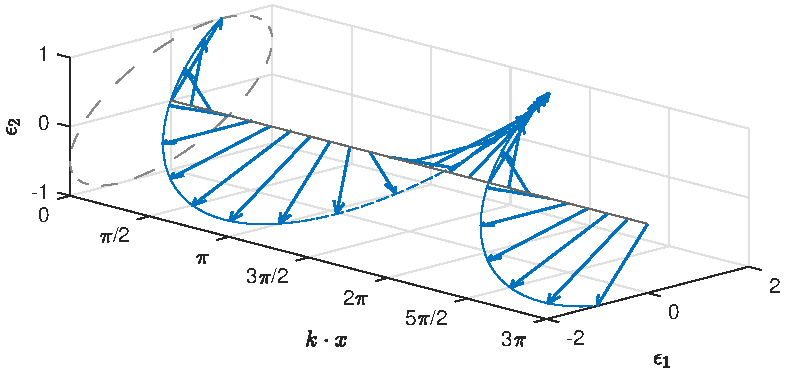
\includegraphics[width=0.5\linewidth]{figures/polarization_elli.pdf}
    \captionof{figure}{椭圆偏振}
    \label{fig:elliptical polarization}
\end{notecaptionblock}
为了方便地描述这个椭圆的方程，记$\Re(\bm E) = E_{\epsilon_1}\uvec\epsilon_1 + E_{\epsilon_2}\uvec\epsilon_2$，则
\begin{align*}
    E_{\epsilon_1} &= \abs{E_1}\cos(\bm k \cdot \bm r - \omega t),\\
    E_{\epsilon_2} &= \abs{E_2}\cos(\bm k \cdot \bm r - \omega t + \delta),
\end{align*}
则
\begin{equation}
    \label{eq:ed-polarization-ellipse}
    \Bigp{\frac{E_{\epsilon_1}}{\abs{E_1}}}^2 + \Bigp{\frac{E_{\epsilon_2}}{\abs{E_2}}}^2 - 2\Bigp{\frac{E_{\epsilon_1}}{\abs{E_1}}}\Bigp{\frac{E_{\epsilon_2}}{\abs{E_2}}}\cos\delta = \sin^2\delta.
\end{equation}
若$E_-$相对$E_+$的相位差是$\alpha$，
则椭圆半长轴与$\uvec\epsilon_1$轴的夹角为$\alpha/2$，且满足
\begin{equation}
    \label{eq:ed-ellipse-orientation}
    \tan\alpha = \frac{2\abs{E_1}\abs{E_2}}{\abs{E_1}^2 - \abs{E_2}^2}\cos\delta.
\end{equation}
椭圆长短轴之比由$E_\pm$幅值之比给出：
\begin{equation}
    \label{eq:ed-polarization-axial-ratio}
    \frac{E_{\max}}{E_{\min}} = \frac{\abs{E_+} + \abs{E_-}}{\abs{E_+} - \abs{E_-}}.%\quad r:=\frac{\abs{E_-}}{\abs{E_+}};
\end{equation}

\paragraph{Stokes参数}

我们如何从观察光束的细节来确定偏振的状态？对于一束光来说，
\[
    \uvec\epsilon_1 \cdot \bm E,\quad\uvec\epsilon_2 \cdot \bm E;\quad\uvec\epsilon_+\conj \cdot \bm E,\quad\uvec\epsilon_-\conj \cdot \bm E,
\]
分别是沿$\uvec\epsilon_{1,2}$方向线偏振的、左旋和右旋圆偏振的振幅。这些振幅的平方给出了各类偏振强度的一种测量。%为体现幅值和相位因素，记
%我们给出相对于线偏振基和相对于圆偏振基的 Stokes 参数的定义，把这些参数用投影振幅(7.25)来表示，并且还直接用诸分量的幅值和相对位相来表示.为了达到后一目的，我们把(7.19)和(7.24)中的各标量系数定义为一

\begin{definition}
    {Stokes参数}{Stokes parameter}
    在线偏振基$\uvec\epsilon_{1,2}$下，Stokes参数表示为
    \begin{subequations}
        \begin{align}
            s_0 &= \abs{\uvec\epsilon_1 \cdot \bm E}^2 + \abs{\uvec\epsilon_2 \cdot \bm E}^2 = \abs{E_1}^2 + \abs{E_2}^2,\\
            s_1 &= \abs{\uvec\epsilon_1 \cdot \bm E}^2 - \abs{\uvec\epsilon_2 \cdot \bm E}^2 = \abs{E_1}^2 - \abs{E_2}^2,\\
            s_2 &= 2\Re\bigb{(\uvec\epsilon_1 \cdot \bm E)\conj(\uvec\epsilon_2 \cdot \bm E)} = 2\abs{E_1}\abs{E_2}\cos\delta,\\
            s_3 &= 2\Im\bigb{(\uvec\epsilon_1 \cdot \bm E)\conj(\uvec\epsilon_2 \cdot \bm E)} = 2\abs{E_1}\abs{E_2}\sin\delta;
        \end{align}
    \end{subequations}
    在圆偏振基$\uvec\epsilon_\pm$下，Stokes参数表示为
    \begin{subequations}
        \begin{align}
            s_0 &= \abs{\uvec\epsilon_+\conj \cdot \bm E}^2 + \abs{\uvec\epsilon_-\conj \cdot \bm E}^2 = \abs{E_+}^2 + \abs{E_-}^2,\\
            s_1 &= 2\Re\bigb{(\uvec\epsilon_+\conj \cdot \bm E)\conj(\uvec\epsilon_-\conj \cdot \bm E)} = 2\abs{E_+}\abs{E_-}\cos\alpha,\\
            s_2 &= 2\Im\bigb{(\uvec\epsilon_+\conj \cdot \bm E)\conj(\uvec\epsilon_-\conj \cdot \bm E)} = 2\abs{E_+}\abs{E_-}\sin\alpha,\\
            s_3 &= \abs{\uvec\epsilon_+\conj \cdot \bm E}^2 - \abs{\uvec\epsilon_-\conj \cdot \bm E}^2 = \abs{E_+}^2 - \abs{E_-}^2.
        \end{align}
    \end{subequations}
\end{definition}
\begin{corollary}
    Stokes参数仅依赖于$\abs{E_1},\abs{E_2},\delta$或$\abs{E_+},\abs{E_-},\alpha$三个参数，因此并不独立：
    \begin{equation}
        \label{eq:ed-pure-stokes-constraint}
        s_0^2 = s_1^2 + s_2^2 + s_3^2.
    \end{equation}
\end{corollary}

\begin{table}[h]
    \centering
    \caption{典型偏振的Stokes参数}
    \begin{tabular}{ccc}
        \toprule
        偏振 & 取向 & Stokes参数\\
        \midrule
        \multirow{2}{*}{线偏振} & 水平(horizontal)和垂直(vertical) & $[1\enspace \pm 1\enspace0\enspace0]$ \\
         & $\pm\ang{45}$ & $[1\enspace0\enspace \pm 1\enspace0]$ \\
        圆偏振 & 右旋和左旋 & $[1\enspace0\enspace0\enspace \pm 1]$ \\
        \bottomrule
    \end{tabular}
    \label{tab:Stokes parameters}
\end{table}

现实中，即使是%目前应用的
单色性(monochromatic)很好的辐射波束也是由有限波列(finite wave trains)叠加成的，因而根据Fourier定理，它包含一个频率范围，即不完全是单色的。%一种看法认为$a_i,\delta_i$随时间变化缓慢，
这时可观测的Stokes参数就是在一个较长时间尺度上的平均，比如：
\[
    s_2 = 2\ave{a_1a_2\cos(\delta_2 - \delta_1)},
\]
求平均的结果是：准单色波束的Stokes参数满足不等式：
\begin{equation}
    \label{eq:ed-mixed-stokes-constraint}
    s_0^2 \geqslant s_1^2 + s_2^2 + s_3^2,
\end{equation}
无偏振(unpolarized)光或自然光(natural light)：$\bm E$由无数个无规则取向的偏振光叠加，各方向振幅相同，因此$s_1 = s_2 = s_3 = 0$，Stokes参数为
\[
    [1\enspace0\enspace0\enspace0].
\]

\begin{definition}{偏振度}{}
    定义偏振度是总光强$I_\tot$中椭圆偏振的成分$I_\text{elp}$占比：
    \begin{equation}
        \label{eq:ed-degree-of-polarization}
        P := \frac{I_\text{elp}}{I_\tot} = \frac{\sqrt{s_1^2 + s_2^2 + s_3^2}}{s_0},
    \end{equation}
    显然$0 \leqslant P \leqslant 1$，
\end{definition}

\begin{corollary}
    依偏振度分类：
    \begin{compactitem}
        \item $P = 1$对应完全偏振光；
        \item $P = 0$对应无偏振光；
        \item $0 < P < 1$对应部分偏振光(partially polarized)，这时尽管$\bm E$含有各种振动方向的光矢量，但在某一方向更显著，不难表达为无偏振光和完全偏振光的叠加：
        \begin{equation}
            \label{eq:ed-stokes-mixture}
            \begin{bmatrix}
                s_0\\s_1\\s_2\\s_3
            \end{bmatrix}_\text{pp} = (1 - P)
            \begin{bmatrix}
                s_0\\0\\0\\0
            \end{bmatrix}_\text{unp} + P
            \begin{bmatrix}
                s_0\\s_1'\\s_2'\\s_3'
            \end{bmatrix}_\text{elp}.
        \end{equation}
    \end{compactitem}
\end{corollary}

\paragraph{Stokes参数的测量}

Stokes参数在场强上是二次的，只能通过强度测量来确定，并结合：
\begin{itemize}
    \item 线偏振器(linear polarizer)：利用物质的材料特性让透射光只有沿着特定方向偏振的分量透过；
    \item 1/4波片(quarter waveplate)：利用了晶体的双折射(birefringence)现象\footnote{一束光线进入某些晶体会产生两束折射光。改变入射角，其中一束光在晶体内的光速各向同性，称为o光(ordinary)；而另一束光的光速各向异性，称为e光(extraordinary)。}使得o光和e光产生相位差，控制波片厚度便可以使线偏振光变成圆偏振光。
\end{itemize}
如果线偏振器与入射光偏振方向夹角为$\theta$，波片的相位差为$\phi$，则出射光的光强为
\begin{equation}
    \label{eq:ed-polarimeter-intensity}
    I(\theta,\phi) = \frac12(s_0 + s_1\cos2\theta + s_2\sin2\theta\cos\phi - s_3\sin2\theta\sin\phi),
\end{equation}
由此可以利用线偏振器和1/4波片，通过测量4次出射光强来得到4个Stokes参数：
\begin{compactitem}
	\item 线偏振器$\theta = 0$：$I(0,0) = (s_0 + s_1)/2;$
    \item 线偏振器$\theta = \ang{90}$：$I(\ang{90},0) = (s_0 - s_1)/2;$
    \item 线偏振器$\theta = \ang{45}$：$I(\ang{45},0) = (s_0 + s_2)/2;$
    \item 线偏振器$\theta = \ang{45} + 1/4$波片：$I(\ang{45},\ang{45}) = (s_0 - s_3)/2.$
\end{compactitem}

\begin{example}
    {Stokes参数的应用：蟹状星云辐射的偏振态}{the Crab nebula}
    在天体物理中，
    蟹状星云中的脉冲星发来的可见光频和射频(radiofrequency)辐射可以用Stokes参数描写偏振态。
    光频辐射显示出微小的线偏振，而$\omega \simeq \qty{2.5e9}{\per\second}$的射频辐射有高度的线偏振。但两个频段均没有圆偏振的迹象。
    这类资料有助于阐明这些迷人天体发出辐射的机理。
\end{example}

\section{反射与透射}

平面电磁波入射(incident)到不同媒质的分界面上会发生反射(reflect)和透射(transmit)\footnote{也称为折射(refract)。}。下面我们研究这种现象的规律。
\begin{notecaptionblock}
	\tikzfigure{reflection-and-transmission}
	\captionof{figure}{入射波、反射波和透射波}
    \label{fig:refraction}
\end{notecaptionblock}

\paragraph{反射定律和折射定律}

入射波、反射波和透射波的波数分别为$k_\incident,k_\reflected,k_\transmitted$。由前文的结论，边界上电场的切向分量是连续的：
\[
    (\bm E_\incident + \bm E_\reflected - \bm E_\transmitted) \times \uvec n = \bm 0.
\]
对于静止的界面和不随时间变化的线性介质，上式对任意$t$均成立，因此入射、反射和透射波的频率相同：
\begin{equation}
    \label{eqn:omegai=omegar=omegat}
    \omega_\incident = \omega_\reflected = \omega_\transmitted = \omega,
\end{equation}
% 式\eqref{eqn:omegai=omegar=omegat}说明，不论光怎样被散射，都具有相同的频率；
又上式对于分界面上的任意一点均成立，故$\bm E_\incident,\bm E_\reflected,\bm E_\transmitted$在分界面上任意一点的相位差均相同，故
% \[
%     \bm k_\incident\cdot\bm r=\bm k_\reflected\cdot\bm r+\delta_\reflected=\bm k_\transmitted\cdot\bm r+\delta_\transmitted.
% \]
% 从前两项可以得到
% \[
%     (\bm k_\incident-\bm k_\reflected)\cdot\bm r=\delta_\reflected,
% \]
% 由内积的投影性质，$\bm r$的终点会扫过一个垂直于$(\bm k_\incident-\bm k_\reflected)$的平面，而$\bm r$的终点正好在分界面上，因此$(\bm k_\incident-\bm k_\reflected)$垂直于分界面：
% \[
%     (\bm k_\incident-\bm k_\reflected)\times\uvec n=\bm 0,
% \]
% 上述关系当然对第三项也适用，因此：
$\bm k_\incident,\bm k_\reflected,\bm k_\transmitted$三线共面，且三者的切向分量相等：
\begin{equation}
    k_\incident\sin\theta_\incident = k_\reflected\sin\theta_\reflected = k_\transmitted\sin\theta_\transmitted,
\end{equation}

\begin{theorem}{反射定律}{}
    入射波与反射波在同一介质中，当然有$k_\incident = k_\reflected$，故入射角$\theta_\incident$和反射角$\theta_\reflected$相等：
    \begin{equation}
        \theta_\incident = \theta_\reflected;
    \end{equation}
\end{theorem}
入射波与折射波在不同介质中，角度的正弦与波数成反比：
\[
    \frac{\sin\theta_\incident}{\sin\theta_\transmitted} = \frac{k_\transmitted}{k_\incident},
\]
但二者频率相同，对波矢同乘$c/\omega$得到一个无量纲参数：
\begin{definition}
    {折射率}{index of refraction}
    将光速与相速度的比值称为折射率(index of refraction)
    \begin{equation}
        n := \frac c{v_\varphi}.
    \end{equation}
\end{definition}
\begin{theorem}{Snell定律}{Snell's law}
    入射角$\theta_\incident$和折射角$\theta_\transmitted$的正弦与折射率成反比：
    \begin{equation}
        \label{eqn:Snell}
        n_\incident\sin\theta_\incident = n_\transmitted\sin\theta_\transmitted.
    \end{equation}
\end{theorem}

\paragraph{电磁分量的变化}

定义振幅的反射系数(reflection coefficient)和透射系数(transmission coefficient)：
\begin{equation}
    \label{eq:ed-fresnel-amplitudes-definition}
    r := \frac{E_\reflected}{E_\incident},\enspace t := \frac{E_\transmitted}{E_\incident}.
\end{equation}

\begin{theorem}
    {Stokes倒逆关系}{Stokes relation}
    定义$r_{ij},t_{ij}$分别表示从介质$i$入射介质$j$的反射系数和透射系数，由光路可逆
    \begin{notecaptionblock}
        \tikzfigure{stokes-relations-i}
        \tikzfigure{stokes-relations-ii}
        \captionof{figure}{Stokes倒逆关系示意图}
    \end{notecaptionblock}
    可得
    \begin{subequations}
        \begin{gather}
            r_{21} = -r_{12}\\
            r_{12}^2 + t_{12}t_{21} = 1.
        \end{gather}
    \end{subequations}
\end{theorem}

由边界上：$\bm D$和$\bm B$法向分量连续，$\bm E$和$\bm H$切向分量连续。我们可以求出$r,t$的表达式。
根据入射面(入射光线与法线确定的平面)与$\bm E_\incident$的关系可以分成两种独立情形：
\begin{figure}[!htp]
    \centering
    \subcaptionbox{垂直极化波}{\tikzfigure{senkrecht-polarization}}
    \subcaptionbox{平行极化波}{\tikzfigure{parallel-polarization}}
    \caption{垂直极化波和平行极化波}
    \label{fig:senkrecht and parallel polarization}
\end{figure}
% 在应用这些边界条件时，可以考虑线偏振的两种独立情况：
\begin{compactenum}
	\item 垂直极化波(senkrecht polarized)：$\bm E_\incident$与入射面垂直(即$\bm E_\incident$垂直纸面向外)%\footnote{在讨论Fresnel公式之前，我们必须指定$\bm E_\incident$的方向。}
	\begin{align*}
        E_\incident + E_\reflected &= E_\transmitted,\\
        H_\incident\cos\theta_\incident - H_\reflected\cos\theta_\reflected &= H_\transmitted\cos\theta_\transmitted,
    \end{align*}
    \item 平行极化波(parallel polarized)：$\bm E_\incident$与入射面平行(或者说$\bm H_\incident$垂直纸面向外)
    \begin{align*}
        E_\incident\cos\theta_\incident - E_\reflected\cos\theta_\reflected &= E_\transmitted\cos\theta_\transmitted,\\
        H_\incident + H_\reflected &= H_\transmitted,
    \end{align*}
\end{compactenum}
电介质通常满足$\mu_\incident = \mu_\reflected \approx \mu_\transmitted \approx \mu_0$，因此$r,t$的表达式为：
\begin{theorem}
    {Fresnel公式}{Fresnel formula}
    对于垂直极化波，$1 + r_\perp = t_\perp$：
    \begin{subequations}
        \begin{align}
            \label{eqn:Fresnel rperp}
            r_\perp &= \frac{n_\incident\cos\theta_\incident - n_\transmitted\cos\theta_\transmitted}{n_\incident\cos\theta_\incident + n_\transmitted\cos\theta_\transmitted},\\%=-\frac{\sin(\theta_\incident-\theta_\transmitted)}{\sin(\theta_\incident+\theta_\transmitted)},\\
            \label{eqn:Fresnel tperp}
            t_\perp &= \frac{2n_\incident\cos\theta_\incident}{n_\incident\cos\theta_\incident + n_\transmitted\cos\theta_\transmitted};%=\frac{2\sin\theta_\incident\sin\theta_\transmitted}{\sin(\theta_\incident+\theta_\transmitted)};
        \end{align}
    \end{subequations}
    对于平行极化波，$1 + r_\parallel = t_\parallel \cdot n_\transmitted/n_\incident$：
    \begin{subequations}
        \begin{align}
            \label{eqn:Fresnel rpara}
            r_\parallel &= \frac{n_\transmitted\cos\theta_\incident - n_\incident\cos\theta_\transmitted}{n_\transmitted\cos\theta_\incident + n_\incident\cos\theta_\transmitted},\\
            \label{eqn:Fresnel tpara}
            t_\parallel &= \frac{2n_\incident\cos\theta_\incident}{n_\transmitted\cos\theta_\incident + n_\incident\cos\theta_\transmitted}.
        \end{align}
    \end{subequations}
\end{theorem}
    
利用Snell定律\eqref{eqn:Snell}，$r,t$便完全由折射率之比$n_\incident/n_\transmitted$与入射角$\theta_\incident$决定。

\begin{example}
    {Brewster角}{Brewster angle}
    对于平行极化波，存在一个特殊的入射角$\theta_\incident$使得$r_\parallel = 0$，%依\eqref{eqn:Fresnel rpara}
    % \[
    %     n_\transmitted\cos\theta_\incident-n_\incident\cos\theta_\transmitted=0,\quad n_\incident\sin\theta_\incident=n_\transmitted\sin\theta_\transmitted.
    %     %n_\transmitted^2\cos i_{\mathrm{B}}=n_\incident\sqrt{n_\transmitted^2-n_\incident^2\sin^2 i_{\mathrm{B}}},
    % \]
    称为Brewster角：
    \begin{equation}
        \label{eqn:Brewster}
        \theta_{\mathrm{B}} = \arctan\Bigp{\frac{n_\transmitted}{n_\incident}}.
    \end{equation}
    在Brewster角下，平行极化波可以发生全透射，因此加了偏振镜的相机可以拍出更通透的照片：
    \begin{itemize}
        \item 空气折射率$n_\incident = 1$，玻璃的折射率$n_\transmitted = 1.5$，得到$\theta_{\mathrm{B}} = \ang{56.31}$；
        \item 水折射率$n_\transmitted = 4/3$，得到$\theta_{\mathrm{B}} = \ang{53.13}$。
    \end{itemize}
    
\end{example}

\paragraph{全反射}

前面的讨论在绝大程度上只限于外反射($n_\incident < n_\transmitted$)，即光疏介质入射光密介质。相反的情况是内反射($n_\incident > n_\transmitted$)，这时$\theta_\incident < \theta_\transmitted$。
当折射角达到$\ang{90}$时，透射波沿界面传播。再增大入射角，光疏侧变为倏逝波，发生全反射(total internal reflection)。由Snell定律，全反射的临界角为
\begin{equation}
    \label{eqn:total reflect}
    \theta_\critical = \arcsin\Bigp{\frac{n_\transmitted}{n_\incident}}.
\end{equation}
发生全反射时，$\theta_\incident > \theta_\critical$，折射角的正弦
\[
    \sin\theta_\transmitted = \frac{n_\incident}{n_\transmitted}\sin\theta_\incident = \frac{\sin\theta_\incident}{\sin\theta_\critical} > 1,
\]
则$\cos\theta_\transmitted$是纯虚的，
\[
    \e^{\i\bm k'\cdot\bm r} = \e^{\i k_\transmitted(x\sin\theta_\transmitted+z\cos\theta_\transmitted)},
\]
此时折射波在光疏介质内仅平行于表面传播，并在垂直方向上呈指数衰减，Poynting矢量的法向分量在时间平均上为0：
\[
    \bm S \cdot \uvec n = \frac12\Re[(\bm E \times \bm H\conj) \cdot \uvec n] = \frac1{2\omega\mu'}\Re[(\bm k' \cdot \uvec n)\abs{\bm E'_0}^2] = 0.
\]

\paragraph{Goos--Hänchen效应}

发生全反射时，光疏介质中的
倏逝波(evanescent wave)在垂直方向上以$\e^{-z/\delta}$衰减，其中
\begin{equation}
    \label{eq:ed-evanescent-penetration}
    \delta\inv = \sqrt{k_\parallel^2 - k_\transmitted^2}
    = k_\incident\sqrt{\sin^2\theta_\incident - \sin^2\theta_\critical}.
\end{equation}
这里$k_\parallel = k_\incident\sin\theta_\incident$是沿界面的波数。
若光束的角谱很窄，且远离临界角，反射系数的相位$\varphi$随$k_\parallel$变化，使反射光束中心沿界面偏移$D = -\p\varphi/\p k_\parallel$。对于垂直极化，代入$r_\perp$的相位得到Goos--Hänchen偏移
\begin{equation}
    \label{eq:ed-goos-haenchen-shift}
    D_\perp \simeq 2\delta\tan\theta_\incident .
\end{equation}

\paragraph{Fresnel菱体}

全反射时两种偏振的反射系数模长都为1，但相位不同。令$m = n_\transmitted/n_\incident < 1$，$\theta = \theta_\incident$。由Fresnel公式，每次反射产生的相对相移$\Delta = \abs{\arg(r_\parallel/r_\perp)}$满足
\[
    \tan\frac{\Delta}{2} = \frac{\cos\theta\sqrt{\sin^2\theta - m^2}}{\sin^2\theta}.
\]
Fresnel菱体让光束经历两次相同的全反射。选$\Delta = \pi/4$，总相移为$\pi/2$，两偏振分量等幅的入射线偏振光便转为圆偏振光。取玻璃到空气的折射率比$m = 1/1.5$，可得内反射角$\ang{50.2}$或$\ang{53.3}$。
图\ref{fig:fresnel-rhomb-path}画出了两次相移发生的位置。
\begin{notecaptionblock}
    \tikzfigure{fresnel-rhomb-path}
    \captionof{figure}{Fresnel 菱体的截面光路。光垂直端面入射，在一对平行的长边界面上各发生一次全反射，最后平行于入射方向出射。$\theta$ 从界面法线量起。}
    \label{fig:fresnel-rhomb-path}
\end{notecaptionblock}

% \paragraph{垂直入射}
% 如果光是垂直界面入射的，$\theta_\incident=\theta_\transmitted=0$，则
% \begin{align*}
%     r&=\frac{n_\incident-n_\transmitted}{n_\incident+n_\transmitted},\\
%     t&=\frac{2n_\incident}{n_\incident+n_\transmitted}.
% \end{align*}

\section{色散}

所有介质都表现出一定的色散性，只有在有限的频率范围内，或在真空中，光的传播速度才能被视为常量。

\paragraph{色散的简单模型}
我们忽略外加电场和局部电场之间的区别。因此，该模型只适用于密度相对较低的物质。
忽略磁场力，
由谐波力束缚和由电场作用的电荷电子的运动方程为：
\[
    -m_\electron\omega_0^2\bm r - m_\electron\gamma\dotbm{r} - e\bm E = m_\electron\ddot{\bm r}.
\]
$-m_\electron\omega_0^2\bm r$是回复力(restoring force)，$-m_\electron\gamma\dotbm{r}$是唯象的阻尼力(damping force)。
如果振荡的振幅足够小，便可以计算电子平均位置的电场。场随频率$\omega$的简谐$\e^{-\i\omega t}$变化。
则由一个电子贡献的偶极矩为：
\[
    \bm p = -e\bm r = \frac{e^2}{m_\electron(\omega_0^2 - \omega^2 - \i\omega\gamma)}\bm E.
\]
从微观到宏观，单位体积内有$N$个分子，每个分子有$Z$个电子；我们将分子中的电子分类，第$j$组有$f_j$个特性相同的电子，其结合频率为$\omega_j$，阻尼常数为$\gamma_j$。
代入$\bm P = \varepsilon_0\chi_\electric\bm E$和$\varepsilon_\relative = 1 + \chi_\electric$得到
\begin{equation}
    \varepsilon_\relative(\omega) = 1 + \frac{Ne^2}{\varepsilon_0m_\electron}\sum_j\frac{f_j}{\omega_j^2 - \omega^2 - \i\omega\gamma_j},
\end{equation}
在量子力学中，$f_j,\omega_j,\gamma_j$都有合适的定义，因此上面的方程准确地描述了原子对介电常数的贡献。我们称$f_j$为振子强度(oscillator strength)，$\omega_j$为共振频率(resonant frequency)。

在远离各共振的频段，$|\omega_j^2 - \omega^2| \gg \omega\gamma_j$，上式可约化为
\[
    \varepsilon_\relative(\omega) \simeq 1 + \frac{Ne^2}{\varepsilon_0m_\electron}\sum_j\frac{f_j}{\omega_j^2 - \omega^2},
\]
对于$\omega < \min(\omega_j)$的低频率下，和的贡献是正的，$\varepsilon_\relative > 1$；随着频率的增加，它将穿过越来越多的$\omega_j$，求和将从正到负，最后$\varepsilon_\relative < 1$。

\paragraph{反常色散和共振吸收}

保留阻尼项，记 $A_j = Ne^2f_j/(\varepsilon_0m_\electron)$，则单个共振对电极化率的贡献为
\begin{equation}
    \label{eq:ed-lorentz-oscillator-susceptibility}
    \chi_j(\omega) = A_j\frac{(\omega_j^2 - \omega^2) + \i\omega\gamma_j}
    {(\omega_j^2 - \omega^2)^2 + \omega^2\gamma_j^2}.
\end{equation}
频率由低到高扫过 $\omega_j$ 时，$\Re\chi_j$ 从正变负，而 $\Im\chi_j$ 在共振附近显著增大。
采用 $\e^{-\i\omega t}$ 的约定时，$\Im\varepsilon_\relative > 0$ 表示电磁波向介质传递能量，由此产生共振吸收(resonant absorption)。

回忆\secref{ssec:Poynting in dissipative media}中线性色散介质中的Poynting定律\eqref{eqn:Poynting with loss}，考虑平面波的衰减(attenuation)，波数是一个复数
\begin{equation}
    \label{eq:ed-complex-propagation-constant}
    k = \beta + \i\frac\alpha 2 = \frac{\omega}{c}(n + \i\kappa).
\end{equation}
这里 $n$ 和消光系数 $\kappa$ 分别是复折射率的实部和虚部。沿 $+z$ 传播时，光强按 $I(z) = I(0)\e^{-\alpha z}$ 衰减。用真空波长 $\lambda_0 = 2\pi c/\omega$ 表示，本章的强度吸收系数为$\alpha \equiv \alpha_I = 4\pi\kappa/\lambda_0 = 2\Im k$，对应的场振幅衰减常数为$\alpha_I/2$。对于非磁性介质，在弱吸收条件 $\alpha \ll \beta$ 下有
\[
    k = \frac\omega c\sqrt{\varepsilon_\relative} \implies
    \begin{cases}
        \alpha \simeq \frac{\Im(\varepsilon_\relative)}{\Re(\varepsilon_\relative)}\beta,\\
        \beta \simeq \frac\omega c\sqrt{\Re(\varepsilon_\relative)}.
    \end{cases}
\]

\paragraph{低频表现，电导}

在低频极限$\omega \to 0$下，如果每个分子中电子的某些$f_0$是自由的，即$\omega_0 = 0$，则$\varepsilon_\relative$在$\omega = 0$处是奇异的。

如果自由电子的贡献被分别显示出来，
\[
    \varepsilon(\omega) = \varepsilon_{\mathrm{b}}(\omega) + \i\frac{Ne^2f_0}{m_\electron\omega(\gamma_0 - \i\omega)},
\]
其中$\varepsilon_{\mathrm{b}}$体现其他偶极子的贡献。

\begin{definition}{电导率}{conductivity}
    引入电导率(conductivity) $\sigma$的概念，体现电流密度与电场强度的关系：
    \begin{equation}
        \bm J = \sigma\bm E,
    \end{equation}
    这也称为Ohm定律($I = U/R$)的微观表达式。
\end{definition}
式\eqref{eqn:Maxwell curlH freq}变为
\[
    \curl\bm H = \sigma\bm E - \i\omega\bm D.
\]
而$\bm D = \varepsilon_{\mathrm{b}}\bm E$，
故电导率也是一个复数：
\begin{equation}
    \sigma = \frac{f_0Ne^2}{m_\electron(\gamma - \i\omega)},
\end{equation} 
\begin{example}{铜的电导率}{conductivity of copper}
    铜的参数为
    \begin{align*}
        N &= \qty{8e28}{\per\metre\cubed},\\
        \sigma &= \qty{5.9e7}{\per\ohm\per\metre}.
    \end{align*}
    由此得到$\gamma_0/f_0 \simeq \qty{4e13}{\per\second}$，而$f_0 \sim 1$，因此当$\omega \leqslant \qty{e11}{\per\second}$时，铜的导电率是实数，并且与频率无关。
\end{example}

\paragraph{高频极限，等离子体频率}

在$\omega \gg \max(\omega_j)$的高频下，
\begin{equation}
    \label{eq:ed-plasma-permittivity-asymptote}
    \varepsilon_\relative(\omega) \simeq 1 - \frac{\omega_{\mathrm{p}}^2}{\omega^2},
\end{equation}
$\omega_{\mathrm{p}}$是介质的等离子体频率(plasma frequency)
\begin{equation}
    \omega_{\mathrm{p}}^2 = \frac{NZe^2}{\varepsilon_0m_\electron},\quad Z = \sum_jf_j.
\end{equation}
仅取决于总电子密度$NZ$。
\begin{example}{地球电离层的短波全反射}{ionisphere}
    用冷等离子体近似电离层的一个均匀层，忽略电子碰撞和地磁场。对垂直入射的波，当 $\omega < \omega_{\mathrm p}$ 时，
    \[
        ck = \omega\sqrt{\varepsilon_\relative} = \sqrt{\omega^2 - \omega_{\mathrm{p}}^2}.
    \]
    是纯虚数。入射波遇到这样的半无限层会全反射，层内场振幅按 $\exp[-\Im(k)z]$ 衰减。
    这里的衰减来自截止产生的倏逝场，在该无碰撞模型中耗散功率为零。

    取 F 层典型的自由电子数密度 $NZ = \qty{e12}{\per\metre\cubed}$，
    则 $\omega_{\mathrm p} \simeq \qty{5.6e7}{\per\second}$，对应的截止频率
    $f_{\mathrm p} = \omega_{\mathrm p}/(2\pi) \simeq \qty{9}{\mega\hertz}$。
    \footnote{\href{https://data.ngdc.noaa.gov/instruments/remote-sensing/active/profilers-sounders/ionosonde/documentation/Digisonde/DPS4_Operations_Manual/NewSect1.pdf}{Digisonde 电离层探测仪手册，第 1 章}。}
\end{example}
\begin{example}{无碰撞等离子体中的能量速度}{plasma energy speed}
    在静止、无背景磁场的冷等离子体中，设离子不动，电子数密度为$n_{\mathrm e}$。当$\omega > \omega_{\mathrm p}$时，横波满足$\omega^2 = c^2k^2 + \omega_{\mathrm p}^2$，其相速度$\omega/k > c$。能量以什么速度通过一个截面？
    电子满足$-\i\omega m_\electron\bm v_0 = -e\bm E_0$，故单位体积电子的周期平均动能为
    \[
        \ave{u_{\mathrm{kin}}} = \frac14 n_{\mathrm e}m_\electron\abs{\bm v_0}^2
            = \frac{\varepsilon_0}4\frac{\omega_{\mathrm p}^2}{\omega^2}\abs{\bm E_0}^2 .
    \]
    由$\abs{\bm B_0} = k\abs{\bm E_0}/\omega$，电场和磁场本身的平均储能为$\varepsilon_0(1 + c^2k^2/\omega^2)\abs{\bm E_0}^2/4$。加上电子动能后，色散关系给出$\ave u = \varepsilon_0\abs{\bm E_0}^2/2$，与\eqref{eqn:Brillouin energy}一致。取沿$+z$传播的波，
    \begin{subequations}
        \label{eq:ed-plasma-energy-velocity}
        \begin{align}
            \ave{S_z} &= \frac{k}{2\mu_0\omega}\abs{\bm E_0}^2,\\
            v_{\mathrm E} &= \frac{\ave{S_z}}{\ave u} = \frac{c^2k}{\omega}
                          = \dv\omega k = v_{\mathrm g}.
        \end{align}
    \end{subequations}
    接近截止时，磁场和能流趋于零，电场和电子仍交替储能。此时群速度也趋于零，而$v_{\mathrm g}v_\varphi = c^2$。
\end{example}
\begin{example}{金属的紫外透射现象}{ultraviolet transparency}
    对于$\omega \ll \omega_{\mathrm{p}}$，光被完全反射；当频率$\omega$增加到$\varepsilon_\relative(\omega) > 0$的区间，金属便突然可以透射光，其反射率变化得很剧烈(drastically)，这称为紫外透射(ultraviolet transparency)现象。
\end{example}

\paragraph{水的折射率和吸收系数随频率的变化}

\figref{fig:water dispersion}比较了 \qty{25}{\degreeCelsius} 液态水在可见光与红外波段的响应。
在绿光 $\lambda_0 = \qty{550}{\nano\metre}$ 处，$n = 1.333$，仅计吸收时，光强衰减至入射值 $1/\e$ 的距离 $1/\alpha$ 约为 \qty{22}{\metre}。
在红外 $\lambda_0 = \qty{2.95}{\micro\metre}$ 处，光激发水分子中 O--H 键的伸缩振动，这一距离缩短至 \qty{0.79}{\micro\metre}。沿右图横轴从低频向高频读，在吸收峰两侧的折射率极大值与极小值之间，$n$ 随频率升高而下降，这就是反常色散。
作图所用的 $\kappa$ 取自 Hale 和 Querry 对实验光谱的汇编和平滑，折射率由作者用减除型 Kramers--Kronig 关系求得。\footnote{光学常数见 G.~M. Hale and M.~R. Querry, \href{https://doi.org/10.1364/AO.12.000555}{\textit{Applied Optics} \textbf{12}, 555--563 (1973)}, Table~I。O--H 伸缩振动的红外光谱见 \href{https://doi.org/10.1038/ncomms9384}{\textit{Nature Communications} \textbf{6}, 8384 (2015)}, Fig.~1。}
\begin{notecaptionblock}
    \includegraphics[width=.90\linewidth]{figures/water_dispersion.pdf}
    \captionof{figure}[液态水的色散与吸收]{液态水的折射率 $n$ 和强度吸收系数 $\alpha$ 随频率 $f = \omega/(2\pi)$ 的变化。左列的绿色区域标出 \qtyrange{400}{700}{\nano\metre} 可见光，蓝灰色区域在右列用线性刻度放大。圆点为文献表值及由其换算的 $\alpha$，连线引导读图。虚线标出该红外吸收带中 $\alpha$ 最大的表列频率。}
    \label{fig:water dispersion}
\end{notecaptionblock}

\sectionstar{在电离层和磁层中的传播模型}

在\exmref{exm:ionisphere}中，电子沿波的电场方向振荡。若存在地磁场，运动电子还受到横向Lorentz力。对于沿地磁场传播的波，两个旋向相反的圆偏振分量将有不同的波数。

\paragraph{沿磁场传播的圆偏振波}
设均匀冷等离子体中有静磁场$\bm B_0 = B_0\uvec z$，取$B_0 > 0$。考虑$\e^{\i(kz-\omega t)}$的微弱横波，频率足够高，可忽略碰撞和离子对波的响应。电子受到波电场和背景磁场的作用，一阶速度满足
\[
    -\i\omega m_\electron\bm v = -e(\bm E + \bm v \times \bm B_0).
\]
令$\Omega_\electron = eB_0/m_\electron$为电子回旋角频率的大小。按前面定义的圆偏振基$\uvec\epsilon_\pm = (\uvec x \pm \i\uvec y)/\sqrt2$，有$\uvec\epsilon_\pm \times \uvec z = \pm\i\uvec\epsilon_\pm$。两个分量各自满足
\begin{align*}
    v_\pm &= \frac{-\i e E_\pm}{m_\electron(\omega \mp \Omega_\electron)},\\
    -\i\omega P_\pm &= J_\pm = -n_\electron e v_\pm.
\end{align*}
其中$n_\electron$为自由电子数密度。由$D_\pm = \varepsilon_0 E_\pm + P_\pm$，两个传播分支的折射率为
\begin{subequations}
    \begin{align}
        n_\pm^2 &= \frac{c^2 k_\pm^2}{\omega^2}
        = 1 - \frac{\omega_{\mathrm p}^2}{\omega(\omega \mp \Omega_\electron)},\\
        \omega_{\mathrm p}^2 &= \frac{n_\electron e^2}{\varepsilon_0m_\electron}.
    \end{align}
\end{subequations}
$B_0 \to 0$时，两支恢复相同的等离子体色散关系。固定$z$观察，$\uvec\epsilon_+$支的电场沿自由电子回旋的方向转动，在$\omega = \Omega_\electron$处产生回旋共振。在共振附近计算有限的吸收率时，需要计入阻尼或电子速度分布。

\paragraph{Faraday旋转}
设入射波沿$x$偏振，且两个圆偏振分量均可无损传播。它们的振幅相等，经过距离$L$后分别积累相位$k_+L$和$k_-L$。将两项相加，略去公共相位，偏振方向成为$\uvec x\cos\psi + \uvec y\sin\psi$，其中
\begin{equation}
    \label{eq:ed-faraday-rotation}
    \psi = \frac{k_- - k_+}2 L.
\end{equation}
在$\omega \gg \omega_{\mathrm p},\Omega_\electron$时展开上式，得到
\begin{equation}
    \psi \simeq \frac{\omega_{\mathrm p}^2\Omega_\electron L}{2c\omega^2}.
\end{equation}
旋转角与真空波长的平方成正比。对于电子密度和纵向磁场沿路径缓慢变化的情形，应将$\omega_{\mathrm p}^2\Omega_\electron L$换为路径积分，回旋频率取$eB_z/m_\electron$的代数值。因此不同波长的偏振角可用来测量沿途$n_\electron B_z$的积分。

\paragraph{Alfvén波}
在远低于离子回旋频率的长波极限下，离子也随场运动，惯性主要来自离子。用理想导电的单流体描述密度均匀的等离子体。设其质量密度为$\rho_{\mathrm m}$，横向流速扰动$\bm u_\perp$和磁场扰动$\bm b_\perp$仅依赖于$z,t$。忽略位移电流，由$\bm J \times \bm B_0$给出的力密度以及理想导体条件$\bm E = -\bm u_\perp \times \bm B_0$，分别得到
\begin{subequations}
    \label{eq:ed-alfven-first-order}
    \begin{align}
        \rho_{\mathrm m}\pv{\bm u_\perp}t &= \frac{B_0}{\mu_0}\pv{\bm b_\perp}z,\\
        \pv{\bm b_\perp}t &= B_0\pv{\bm u_\perp}z.
    \end{align}
\end{subequations}
消去$\bm b_\perp$即得沿背景磁场传播的横波
\begin{subequations}
    \begin{align}
        \pv[2]{\bm u_\perp}t &= v_{\mathrm A}^2\pv[2]{\bm u_\perp}z,\\
        v_{\mathrm A} &= \frac{B_0}{\sqrt{\mu_0\rho_{\mathrm m}}}.
    \end{align}
\end{subequations}
弯曲磁力线产生的磁张力提供回复力，流体惯性决定其加速度。上式给出的Alfvén速度适用于$v_{\mathrm A} \ll c$、电阻扩散可忽略的情形。

\section{群速度}

如果介质是色散的，则波的每个频率分量的相速度都不相同，能流的速度可能与相位的速度有很大的不同，甚至缺乏精确的意义。

\paragraph{一维标量波}

一维均匀介质中，固定频率的标量波可写为
\[
    u(x,t) = a\e^{\i(kx-\omega t)} + b\e^{\i(-kx-\omega t)},
\]
由色散性质，$\omega = \omega(k)$是波数的函数。将标量波表示成Fourier变换的形式
\[
    u(x,t) = \frac1{\sqrt{2\pi}}\intR A(k)\e^{\i(kx-\omega t)}\d k,
\]
$A(k)$描述了不同波的线性叠加的性质，
\[
    A(k) = \frac1{\sqrt{2\pi}}\intR u(x,0)\e^{-\i kx}\d x,
\]
对于一个单色行波，$u(x,0) \sim \e^{\i k_0x}$，则$A(k) = \sqrt{2\pi}\delta(k - k_0)$，从而$u(x,t) = \e^{\i(k_0x-\omega_0t)}$。

\paragraph{有限波列、群速度}

对于一个有限波列(wave train)，$x,k$平均值的均方根偏差$\Delta x,\Delta k$满足Fourier带宽(bandwidth)定律
\begin{equation}
    \Delta x\Delta k \geqslant \frac12,
\end{equation}
如果一个脉冲的波数谱不太广，或者一个介质中的频率对波数的依赖性较弱，则$\omega(k)$可以被展开
\[
    \omega(k) = \omega_0 + \biggeval{\dv\omega k}_0(k - k_0) + \cdots
\]
得到 
\[
    u(x,t) \simeq u\Bigp{x - t\biggeval{\dv\omega k}_0,0}\exp\biggb{\i\Bigp{k_0\biggeval{\dv\omega k}_0 - \omega_0}t},
\]
除了一个整体的相位因子，脉冲以一种没有失真的(undistorted)速度传播，称为群速度(group velocity)
\begin{equation}
    v_{\mathrm{g}} := \biggeval{\dv\omega k}_0,
\end{equation}
对于光波，以折射率$n(k)$表示更方便：
\[
    \omega(k) = \frac{ck}{n(k)},
\]
相速度
\begin{equation}
    \label{eq:ed-phase-velocity-isotropic}
    v_\varphi = \frac{\omega(k)}k = \frac c{n(k)},
\end{equation}
群速度
\begin{equation}
    \label{eq:ed-group-velocity-isotropic}
    v_{\mathrm{g}} = c\biggp{\frac1n - \frac k{n^2}\dv nk} = \frac cn - \frac\omega n\dv n\omega v_{\mathrm{g}},
\end{equation}
得到 
\begin{equation}
    \label{eqn:gruop v}
    v_{\mathrm{g}} = \frac c{\displaystyle n(\omega) + \omega\dv n\omega},
\end{equation}

\paragraph{群速度可以大于光速吗？}

在透明或弱吸收频段，$\d n/\d\omega > 0$称为正常色散，$\d n/\d\omega < 0$称为反常色散(anomalous dispersion)。由式\eqref{eqn:gruop v}，某些反常色散频段的群速度可大于$c$，甚至为负；仅有$\d n/\d\omega < 0$并不足以保证超光速。此时吸收、增益或高阶色散可能显著重塑波包，波包峰值的移动不能直接等同于信息或能量输运。对满足因果性且高频极限$n(\omega) \to 1$的局域电磁响应，携带新扰动的信号前沿仍不超越真空光速$c$。

\paragraph{进一步讨论群速度的有效性}

对满足$\ddot{\hat u}(k,t) + \omega(k)^2\hat u(k,t) = 0$的无损线性模型，设初值为$f(x) = u(x,0)$、$g(x) = \dot u(x,0)$，并以$\hat f,\hat g$表示同一归一化约定下的Fourier变换。保留两个时间分支后，解为
\[
    u(x,t) = \frac1{\sqrt{2\pi}}\intR
    \biggb{\hat f(k)\cos\bigp{\omega(k)t}
    + \hat g(k)\frac{\sin\bigp{\omega(k)t}}{\omega(k)}}\e^{\i kx}\d k.
\]
若$\omega(k) = 0$，其中$\sin(\omega t)/\omega$取连续极限$t$。令$t = 0$并对$t$求导，即可分别恢复两项初始条件。
\begin{example}{Gauss波包}{Gaussian modulated oscillation}
    考虑初始为Gauss调制振荡：
    \[
        f(x) = \e^{-x^2/2L^2}\cos(k_0x),\qquad g(x) = 0.
    \]
    其Fourier谱为
    \[
        \hat f(k) = \frac L2\bigb{\e^{-L^2(k-k_0)^2/2} + \e^{-L^2(k+k_0)^2/2}},
    \]
    故演化由
    \[
        u(x,t) = \frac1{\sqrt{2\pi}}\intR\hat f(k)\cos\bigp{\omega(k)t}\e^{\i kx}\d k
    \]
    给出。零初速度一般同时激发两个时间分支，不能直接用单个平移波包代替此解。
    \tcblower
    例如，选取偶对称的模型色散关系
    \[
        \omega(k) = \omega_\ast\Bigp{1 + \frac{a^2k^2}2},
    \]
    其中$\omega_\ast$是角频率、$a$是长度，则正频率分支在$k_0$附近的群速度为
    \[
        v_{\mathrm{g}} = \biggeval{\dv\omega k}_{k_0} = \omega_\ast a^2k_0.
    \]
    此式量纲为速度；二阶导数$\omega''(k) = \omega_\ast a^2$还会使窄带波包展宽。
\end{example}

\paragraph{Gauss脉冲的时间展宽}
在实验中，常在固定位置记录一个单向传播的脉冲随时间的变化。设$x = 0$处的复场为$u(0,t) = A_0\e^{-t^2/(2T_0^2)}\e^{-\i\omega_0t}$，初始包络没有啁啾。介质在脉冲带宽内透明，且带宽远小于$\omega_0$。记$\Omega = \omega - \omega_0$，将波数展开到二阶，
\begin{equation}
    \label{eq:ed-dispersion-expansion-frequency}
    k(\omega_0 + \Omega) \simeq k_0 + \frac{\Omega}{v_{\mathrm g}} + \frac12 k''_0\Omega^2.
\end{equation}
这里$k''_0 = \biggeval{\dv[2]k\omega}_{\omega_0}$。
在传播距离$x$内，若三阶及更高阶色散积累的相位在脉冲带宽内均可忽略，一次项使包络中心推迟$x/v_{\mathrm g}$，二次项使不同频率分量获得不同的群延迟。取$\tau = t - x/v_{\mathrm g}$，并从复场中提出载波因子$\e^{\i(k_0x-\omega_0t)}$，剩下的包络为
\begin{align*}
    A(x,\tau)
    &= \frac{A_0 T_0}{\sqrt{2\pi}}\intR
    \exp\biggb{-\frac{T_0^2 - \i k''_0x}{2}\Omega^2 - \i\Omega\tau}\d\Omega\\
    &= \frac{A_0}{\sqrt{1 - \i s}}\exp\biggb{-\frac{\tau^2}{2T_0^2(1 - \i s)}},
    \qquad s = \frac{k''_0x}{T_0^2}.
\end{align*}
强度包络正比于$\abs{A}^2$，其半高全宽为
\begin{equation}
    \Delta t(x) = 2\sqrt{\ln 2}\,T_0
        \sqrt{1 + \biggp{\frac{k''_0x}{T_0^2}}^2}.
\end{equation}
脉冲传播一个色散长度$L_{\mathrm D} = T_0^2/\abs{k''_0}$后，宽度增至原来的$\sqrt2$倍。对于这里的无初始啁啾脉冲，$k''_0$的两种符号给出相同的展宽，却使瞬时频率沿脉冲前后以相反的次序排列。若入射脉冲已有啁啾，可选择累积色散$k''_0x$的符号与大小以压缩脉冲。

\section{\texorpdfstring{$\bm D$}{D}和\texorpdfstring{$\bm E$}{E}之间的因果关系}

静态电磁场
\[
    D_\alpha = \varepsilon_0E_\alpha + P_\alpha - \sum_\beta\pv{Q'_{\alpha\beta}}{x_\beta} + \cdots
\]
若考虑时间，
会发生什么变化？

\paragraph{时间非局域性}

在色散介质中，$\varepsilon(\omega)$对频率$\omega$的依赖会导致$\bm D(\bm r,t)$和$\bm E(\bm r,t)$的临时性非局域联系。对于$\omega$的单色成分，
\[
    \hatbm D(\bm r,\omega) = \varepsilon(\omega)\hatbm E(\bm r,\omega),
\]
Fourier变换得到
\[
    \bm D(\bm r,t) = \frac1{2\pi}\intR\varepsilon(\omega)\biggb{\intR\bm E(\bm r,t')\e^{\i\omega t'}\d t'}\e^{-\i\omega t}\d\omega,
\]
假设积分的次序可以交换，可以得到
\begin{equation}
    \label{eqn:D-E with omega}
    \bm D(\bm r,t) = \varepsilon_0\biggb{\bm E(\bm r,t) + \intR\bm E(\bm r,t - \tau)G(\tau)\d\tau},
\end{equation}
其中 
\begin{equation}
    \label{eq:ed-dielectric-memory-kernel}
    G(\tau) = \frac1{2\pi}\intR\bigb{\varepsilon_\relative(\omega) - 1}\e^{-\i\omega\tau}\d\omega,
\end{equation}
因此$t$时刻的$\bm D(\bm r,t)$依赖除$t$以外的电场$\bm E(\bm r,t - \tau)$。若$\varepsilon$是不依赖于$\omega$的，则
\begin{align*}
    G(\tau) &= (\varepsilon_\relative - 1)\delta(\tau),\\
    \bm D(\bm r,t) &= \varepsilon\bm E(\bm r,t),
\end{align*}
$\bm D(\bm r,t)$和$\bm E(\bm r,t)$有瞬时的联系；但如果$\varepsilon(\omega)$随$\omega$变化，则$G(\tau)$在$\tau \neq 0$的一些地方也不会消失。

\paragraph{$G(\tau)$的简单模型}

假设所有的电子都以一个频率$\omega_0$振荡，则 
\[
    \varepsilon_\relative(\omega) = 1 + \frac{\omega_{\mathrm{p}}^2}{\omega_0^2 - \omega^2 - \i\gamma\omega},
\]
即 
\[
    G(\tau) = \frac{\omega_{\mathrm{p}}^2}{2\pi}\intR\frac{\e^{-\i\omega\tau}\d\omega}{\omega_0^2 - \omega^2 - \i\gamma\omega}.
\]
被积函数在$\omega$的下半平面上有两个奇点
\[
    \omega_\pm = -\i\frac\gamma 2 \pm \nu_0,\quad\nu_0^2 = \omega_0^2 - \frac{\gamma^2}4.
\]
利用复变函数中对留数的处理，得到
\begin{equation}
    \label{eq:ed-causal-lorentz-kernel}
    G(\tau) = \omega_{\mathrm{p}}^2\frac{\sin\nu_0\tau}{\nu_0}\e^{-\gamma\tau/2},\quad\tau > 0.
\end{equation}
欠阻尼时，响应的振幅包络按$\e^{-\gamma\tau/2}$衰减，衰减时间为$2/\gamma$。若材料含有多个振子，各自的频率和阻尼共同决定响应延续的时间。

上面的方程在时间(而非空间)上是非局部的。

\paragraph{$\varepsilon(\omega)$的因果性和分析性域}

$\tau < 0$时$G(\tau) = 0$。说明只有在$t$时间之前的电场$\bm E$进入以确定电位移$\bm D$，这符合我们在物理现象中的因果关系的基本思想。

假设：空间局域、线性、因果关系，均匀各向同性介质。


\paragraph{Kramers--Kronig关系}
下式假定$\varepsilon_\relative(\omega) - 1$在复频率上半平面解析、在无穷远充分衰减，且实轴上没有需要另行分离的极点（例如直流电导引起的零频极点）。
由Cauchy定理
\begin{align*}
    \varepsilon_\relative(\omega) - 1 &= \frac1{2\pi\i}\oint_C\frac{\varepsilon_\relative(\omega') - 1}{\omega' - \omega}\d\omega'\\
    &= \frac1{2\pi\i}\lim_{\delta\to0^+}\intR\frac{\varepsilon_\relative(\omega') - 1}{\omega' - \omega - \i\delta}\d\omega'
\end{align*}
由Sokhotski--Plemelj定理\footnote{Sokhotski的姓氏在其波兰文著作中写作Sochocki。}
\begin{equation}
    \label{eq:ed-sokhotski-plemelj}
    \lim_{\delta\to0^+}\frac1{x \pm \i\delta} = \PV\Bigp{\frac1x} \mp \i\pi\delta(x),
\end{equation}
故
\[
    \varepsilon_\relative(\omega) = 1 + \frac1{\pi\i}\PV\intR\frac{\varepsilon_\relative(\omega') - 1}{\omega' - \omega}\d\omega'
\]
由$\Re[\varepsilon_\relative(\omega)]$为偶，$\Im[\varepsilon_\relative(\omega)]$为奇，得到Kramers--Kronig关系
\begin{equation}
    \begin{aligned}
        \Re[\varepsilon_\relative(\omega)] &= 1 + \frac1\pi\PV\intR\frac{\Im[\varepsilon_\relative(\omega')]}{\omega' - \omega}\d\omega'\\
        \Im[\varepsilon_\relative(\omega)] &= -\frac1\pi\PV\intR\frac{\Re[\varepsilon_\relative(\omega')] - 1}{\omega' - \omega}\d\omega'\\
    \end{aligned}
\end{equation}
或
\begin{equation}
    \begin{aligned}
        \Re[\varepsilon_\relative(\omega)] &= 1 + \frac2\pi\PV\intRplus\frac{\omega'\Im[\varepsilon_\relative(\omega')]}{\omega'^2 - \omega^2}\d\omega'\\
        \Im[\varepsilon_\relative(\omega)] &= -\frac{2\omega}\pi\PV\intRplus\frac{\Re[\varepsilon_\relative(\omega')] - 1}{\omega'^2 - \omega^2}\d\omega'\\
    \end{aligned}
\end{equation}
Kramers--Kronig关系将响应函数的实部与虚部联系起来，其物理基础是因果性；具体积分形式还依赖上述解析性、收敛性及奇点处理条件。

例如，在正频率$\omega_0$处有一条非常窄的吸收线。将它近似为$\delta$函数，由第一条关系可得该谱线两侧的色散
\begin{align*}
    \Im[\varepsilon_\relative(\omega)] &\simeq \frac{\pi K}{2\omega_0}\delta(\omega - \omega_0) + \cdots\\
    \Re[\varepsilon_\relative(\omega)] &\simeq \bar\varepsilon + \frac K{\omega_0^2 - \omega^2}.
\end{align*}
其中$\bar\varepsilon$为其余谱线在该频段给出的平滑背景。

\paragraph{介电响应的求和规则}
对无直流电导的被动介质，若静态介电常数有限，在第一条Kramers--Kronig关系中令$\omega = 0$即得
\begin{equation}
    \label{eq:ed-static-dispersion-sum}
    \varepsilon_\relative(0) - 1
    = \frac2\pi\intRplus\frac{\Im[\varepsilon_\relative(\omega')]}{\omega'}\d\omega'.
\end{equation}
相同面积的吸收线，频率越低，对静态极化的贡献越大。另一方面，在上半平面取纯虚频率$\i\xi$，因果响应的积分表示给出
\begin{equation}
    \label{eq:ed-imaginary-frequency-permittivity}
    \varepsilon_\relative(\i\xi) - 1
    = \frac2\pi\intRplus\frac{\omega'\Im[\varepsilon_\relative(\omega')]}{\omega'^2 + \xi^2}\d\omega',
    \qquad \xi > 0.
\end{equation}
在本章的电子振子模型中，$\xi^2[\varepsilon_\relative(\i\xi) - 1] \to \omega_{\mathrm p}^2$。将积分式乘以$\xi^2$并取$\xi \to \infty$，便得到吸收谱的总权重
\begin{equation}
    \intRplus\omega'\Im[\varepsilon_\relative(\omega')]\d\omega'
    = \frac\pi2\omega_{\mathrm p}^2.
\end{equation}
固定总电子数密度$NZ$时，改变振子的回复力或阻尼会改变谱线的位置或宽度，保留这个加权积分。

